\pagenumbering{arabic}

\chapter{Introduction} \label{introduction}

\quad This document is written to describe the Software Requirements Specification (SRS) \cite{8559686} for the open-source project FarmBot. FarmBot is an open-source CNC (computer numerical control) farming project. It consists of a cartesian coordinate robot farming machine, software, and documentation, which includes a farming data repository.

\section{Purpose of the System }
The project aims to create open-source and accessible technology for people to grow food easily. In addition to that, the mission of the benefit corporation FarmBot Inc. is to build a community that develops open-source hardware plans, software, data, and documentation that is available to everyone for building their farming machine. The system, therefore, paves the way for decentralization and democratization of food production.

\section{Scope}

FarmBot is an open-source CNC farming project. The system aims to address the issues that have become prevalent with the ever-growing world population and its food demands. It significantly improves upon the conventional agriculture methods.
The scope of the system consists of the following:
\begin{itemize}
    \item Building a free and open database for farming and gardening knowledge
    \item A custom operating system, FarmBot OS, for maintaining connection and synchronization between the hardware and the web application using message brokers. Allowing scheduling of events, real-time control and uploading various sensor data and logs
    \item A web app for easy configuration and control of the FarmBot, featuring real-time manual control capabilities, logging, drag-and-drop farm designing and a routine builder for FarmBot to execute scheduled routines
    \item Scalability for all sizes of operation from home-use to industrial-use.
    \item Big data acquisition and analysis for data-driven agriculture.
    \item Providing the user with various farm design options with space efficiency in mind
    \item Fully automated and optimized farming operations such as planting, watering, spraying, weed detection, and seed spacing with mono-crop and poly-crop capabilities
    \item Offering customizability to the user in adding new sensors, adjusting parameters of their FarmBot to their liking
\end{itemize}

\begin{figure}[H]
    \centering
    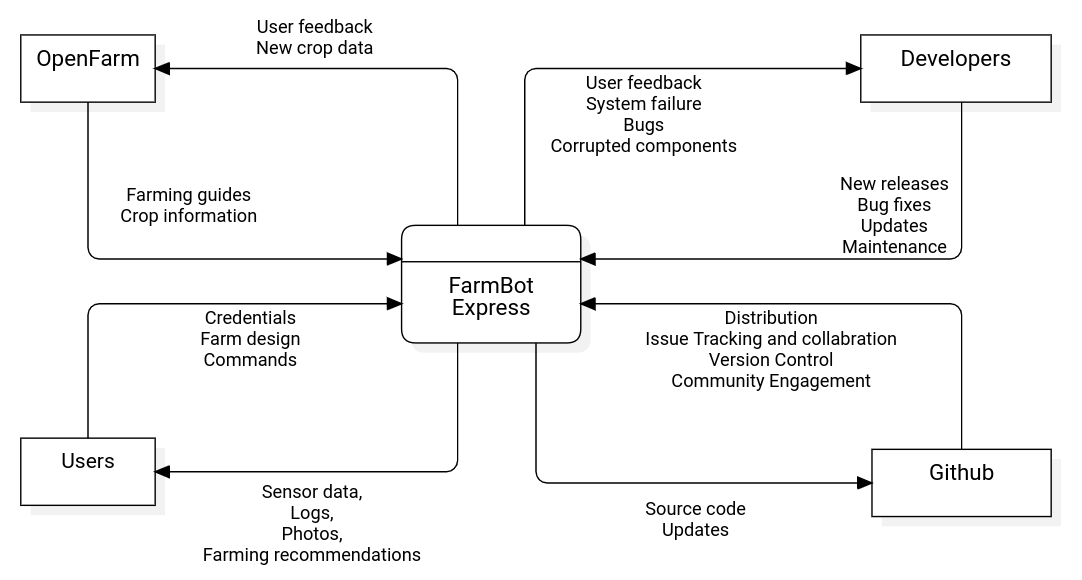
\includegraphics[width=1\textwidth]{UML Diagrams/ContextDiagram.png}
    \caption{Context Diagram}
    \label{fig:context-diagram}
\end{figure}
\subsection{System Perspective}

FarmBot Express is a user-friendly, stand-alone automated gardening system designed to cater to a wide range of users, including beginners, students, researchers, home users, and even individuals with disabilities. This self-contained system leverages a robotic arm controlled by a central computer, a Raspberry Pi. The computer communicates wirelessly with FarmBot's onboard microcontroller, translating digital commands into precise movements for the motors. This enables the versatile 3-in-1 toolhead to perform tasks with high accuracy, such as planting seeds, delivering water directly to plant roots, and even managing weeds with compatible attachments. FarmBot Express integrates sensor systems to monitor environmental factors like soil moisture and temperature, allowing the system to adjust watering schedules for optimal plant growth. While some attachments are sold separately, the ability to detect and manage weeds through these attachments expands FarmBot's overall functionality.

\textbf{Context Diagram Analysis:}

The context diagram provides a high-level overview of how FarmBot Express interacts with its surroundings and the data that flows between them. This visual representation helps to understand the system's functionalities and its role in automating gardening tasks. The core entity is the FarmBot Express system itself, which interacts with three primary external entities:

\textbf{User:} This is the main entity that interacts with FarmBot Express. Users provide various inputs such as credentials for accessing the web interface, farm design data specifying the layout and plant types, and commands to direct the FarmBot's actions.

\textbf{Developer:} This external entitiy is responsible for developing the software and hardware components of FarmBot Express. Developers contribute to the system's functionality by creating new features, improving existing ones, and ensuring compatibility with external systems.

\textbf{Github:} Github is a cloud-based platform that hosts the open-source codebase for FarmBot Express. Developers use Github to collaborate on software development, track changes, and manage version control. The system interacts with Github to access the latest codebase, updates, and documentation.

\textbf{OpenFarm:} OpenFarm is an external database that provides crop information to FarmBot Express. The system communicates with OpenFarm.cc to access detailed plant data, including planting instructions, growth requirements, and other relevant information. This data helps users make informed decisions when designing their farms and scheduling planting tasks.

The data flow between these entities is crucial for the system's operation. Users send information to FarmBot Express, which in turn translates these instructions into actions within the farm environment. Sensor data from the farm is then relayed back to FarmBot Express, allowing the system to monitor and adjust its operations as needed. FarmBot Express may also provide data and recommendations back to the user.


\subsubsection{System Interfaces}

FarmBot Express relies on a network of non-user interfaces to facilitate communication and control between various hardware, software, and communication components. These interfaces can be categorized as internal (within the FarmBot system) and external (between FarmBot and external systems). Communication between these interfaces occurs through established protocols, data formats, and a special operating system FarmBot OS.

\subsubsection{User Interfaces}

FarmBot Express prioritizes user-friendliness by offering intuitive interfaces for interaction and control. These interfaces can be categorized as:
\begin{itemize}

    \item \textbf{Web Interface:} This primary interface acts as the central hub for user interaction with FarmBot Express. Accessible through a web browser on a computer or mobile device, it mainly allows users to:
    
    \textbf{Manage user accounts and profiles:}

    The FarmBot Express Settings page lets users personalize their experience. They can change their password, language, and time format preferences. Additionally, users can choose what information to display in the interface, including sensor data. The page also offers options for managing saved changes, emergency actions, and user interface access restrictions.

    \begin{figure}[H]
        \centering
        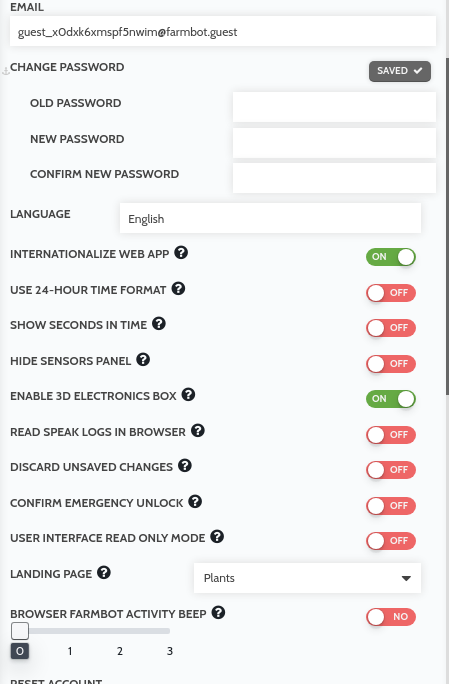
\includegraphics[width=0.6\linewidth]{Figures/ui_user_acc.png}
        \caption{Account Management}
        \label{fig:ui_acc}
    \end{figure}
    
     
    
    \textbf{Create and manage farm profiles (size, layout, settings):}

    FarmBot Express's user interface empowers users to establish and manage detailed profiles for each of their farms. Within these profiles, users can define the farm's size, meticulously map out the garden layout, and configure various settings that optimize FarmBot's operation for that specific plot. This meticulous approach ensures precise automation and efficient resource utilization tailored to the unique needs of each individual farm.

    \begin{figure}[H]
        \centering
        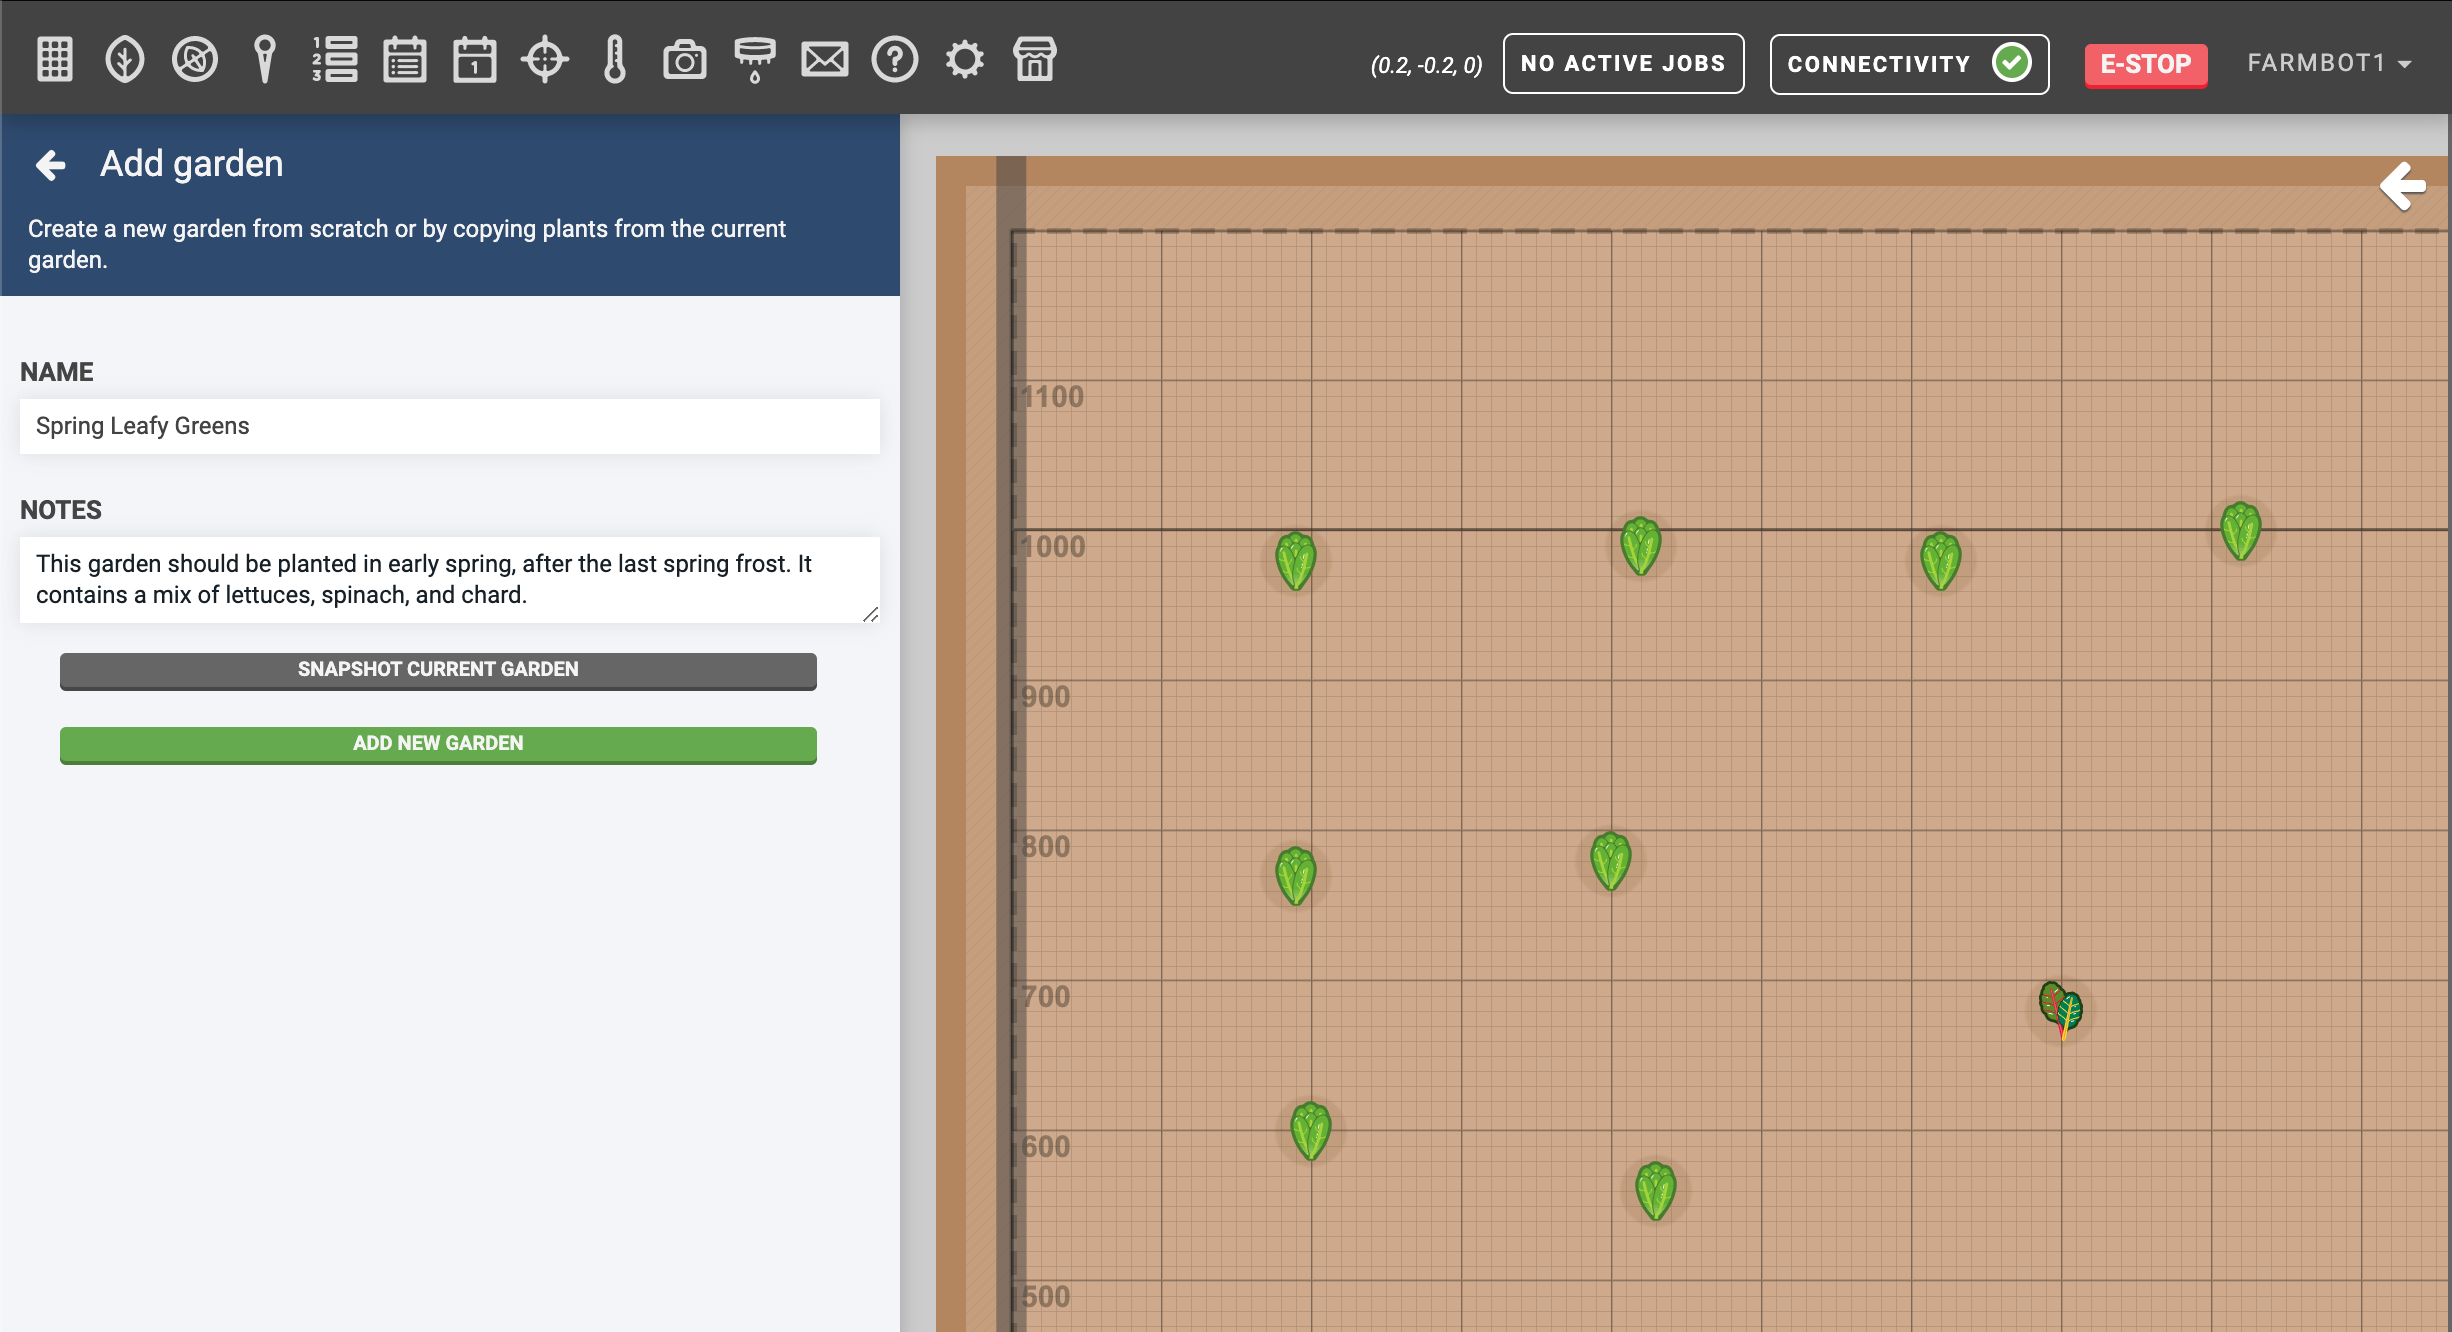
\includegraphics[width=0.5\linewidth]{Figures/ui_addgarden.png}
        \caption{Add Garden}
        \label{fig:garden}
    \end{figure}

    \begin{figure}[H]
        \centering
        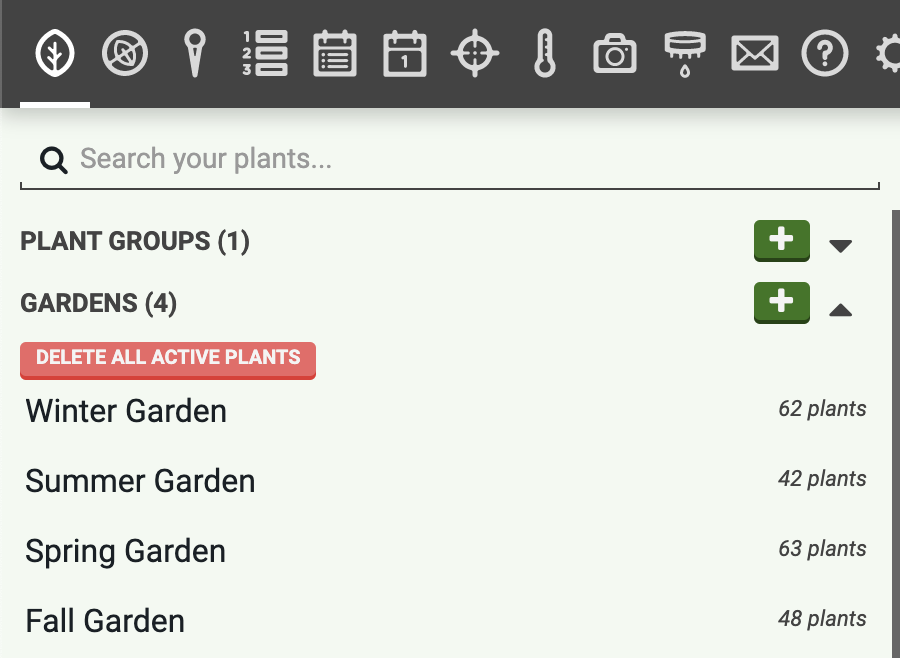
\includegraphics[width=0.5\linewidth]{Figures/ui_viewgarden.png}
        \caption{Garden Profile}
        \label{fig:prof-garden}
    \end{figure}
    
    \textbf{Manual Control:}

    This interface serves as the manual control center for the FarmBot. Notice the directional arrows. One can use these controls to guide a robotic arm across your garden with pinpoint accuracy.  The accompanying numbers (1, 10, 100, 1000, 10000) represent distance increments, allowing for precise movements tailored to the garden's layout and planting needs.
    
    \begin{figure}[H]
        \centering
        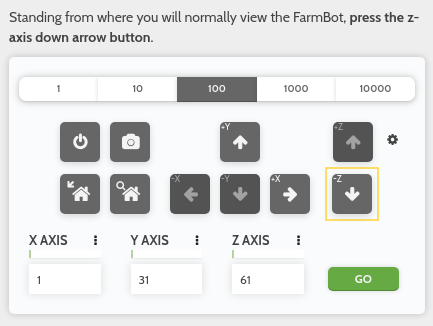
\includegraphics[width=0.6\linewidth]{Figures/ui_mancont.png}
        \caption{Manual Control}
        \label{fig:ui_control}
    \end{figure}

    
    \textbf{Schedule and monitor planting and watering tasks}

    \begin{figure}[H]
        \centering
        \begin{subfigure}{0.49\linewidth}
            \centering
            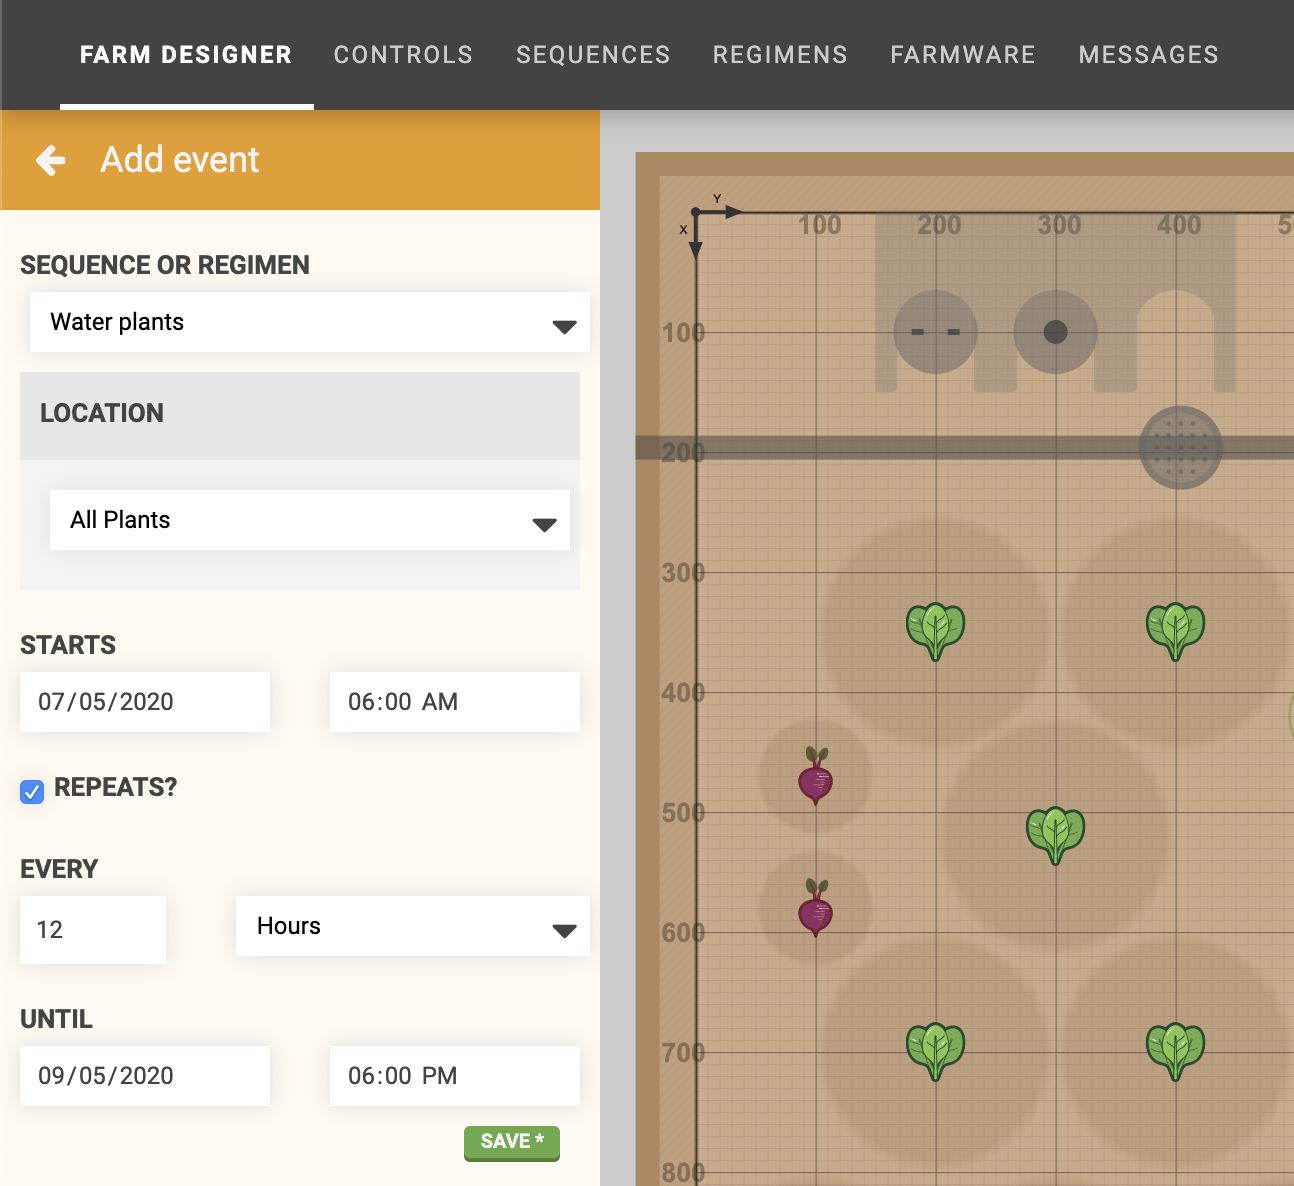
\includegraphics[width=\linewidth]{Figures/ui_schedule.png}
            \label{fig:ui_schedule}
        \end{subfigure}
    \hfill
        \begin{subfigure}{0.49\linewidth}
            \centering
            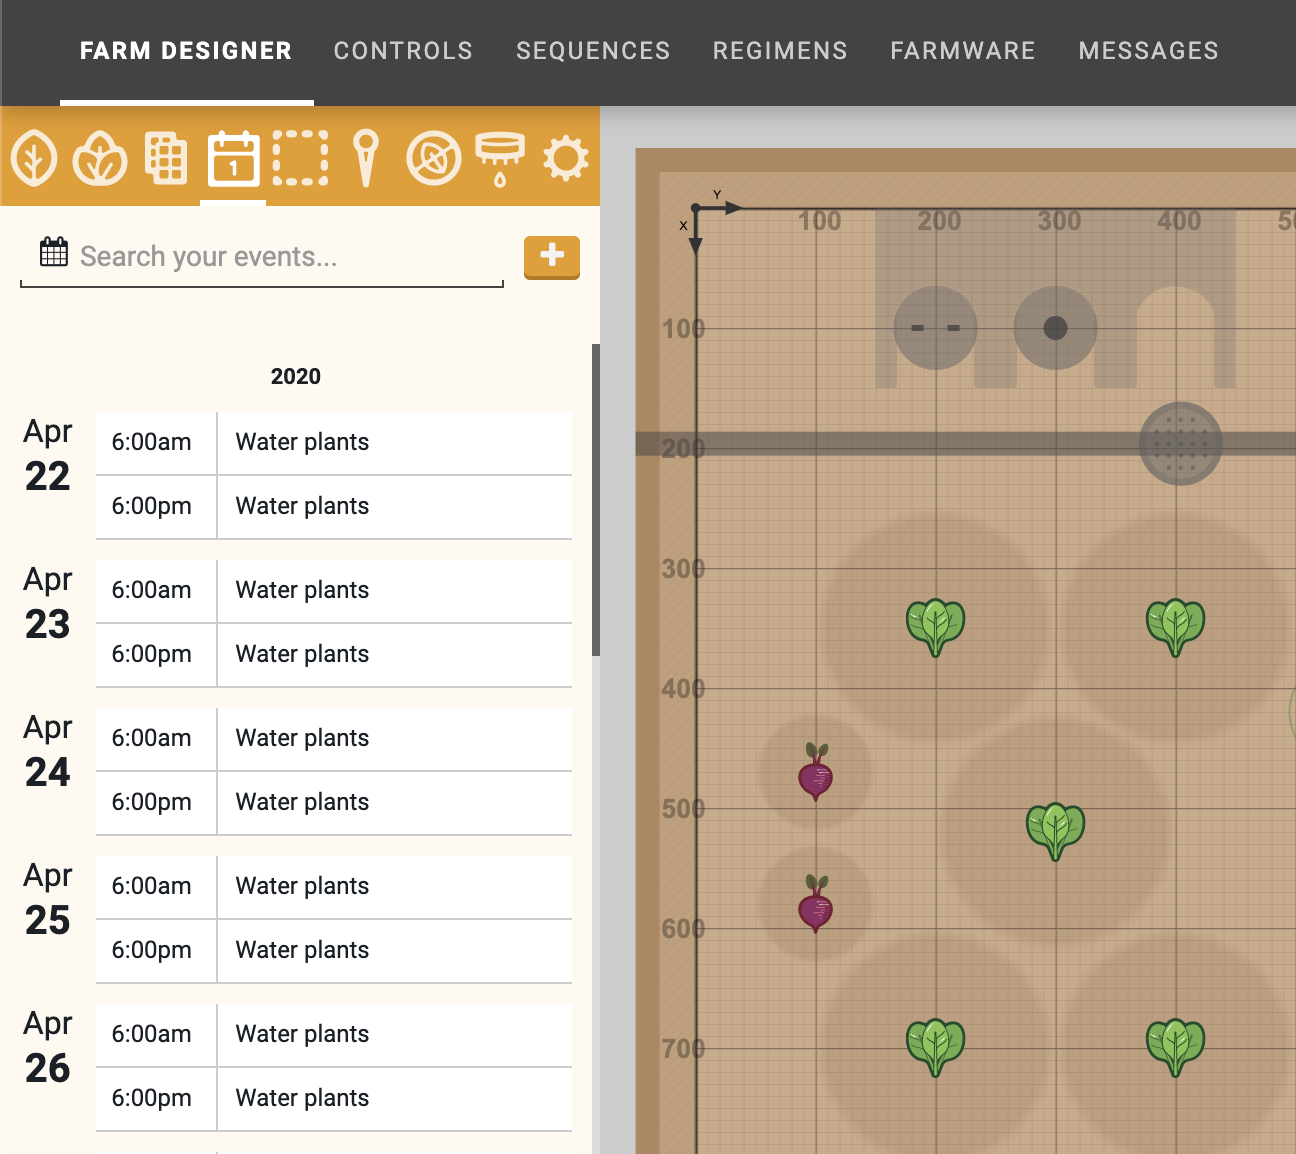
\includegraphics[width=\linewidth]{Figures/ui_sch2.png}
            \label{fig:ui_schedule2}
        \end{subfigure}
    \caption{Event Scheduling}
    \label{fig:event_scheduling}
    \end{figure}

    
    The FarmBot Express Event Scheduler facilitates the creation and management of automated gardening tasks. Users can select the desired action type (e.g., watering, planting), specify the target location (entire garden layout or designated zones), define the start date and time for the event, and configure recurring schedules if necessary. By saving the event details, users can program FarmBot to perform these tasks autonomously, optimizing automated gardening routines.
    

    
    \textbf{Control Peripherals}

    \begin{figure}[H]
        \centering
        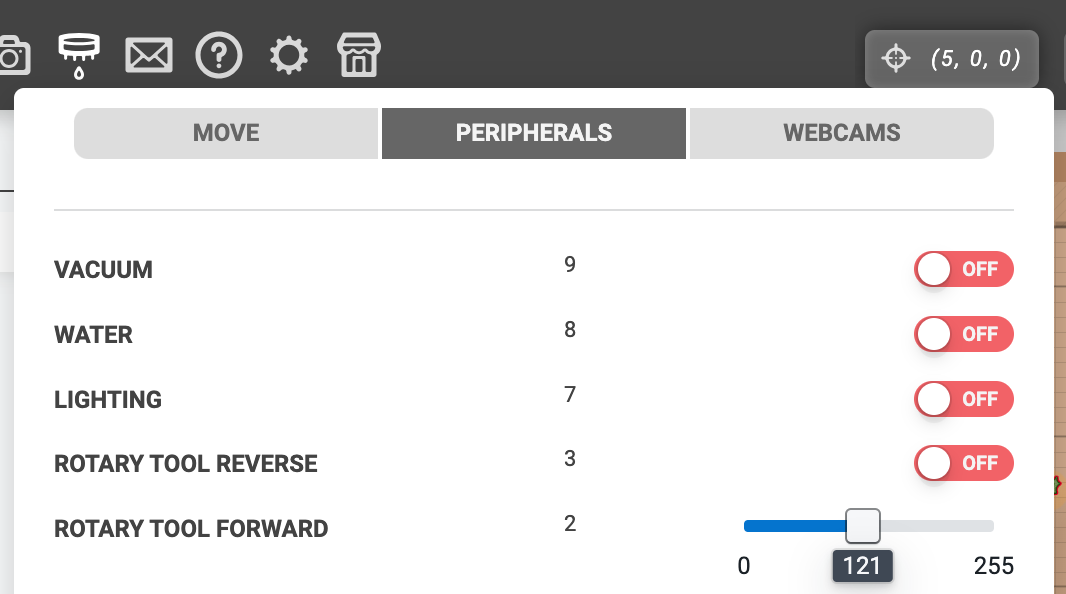
\includegraphics[width=0.6\linewidth]{Figures/ui_peripherals.png}
        \caption{Control Peripherals}
        \label{fig:ui_peri}
    \end{figure}

    The FarmBot Express software provides a dedicated "Peripherals" tab within the control interface. This tab empowers users with real-time control and management of FarmBot's peripheral devices.

    \textbf{Create sequential commands for various tasks}
    
    \begin{figure}[H]
        \centering
        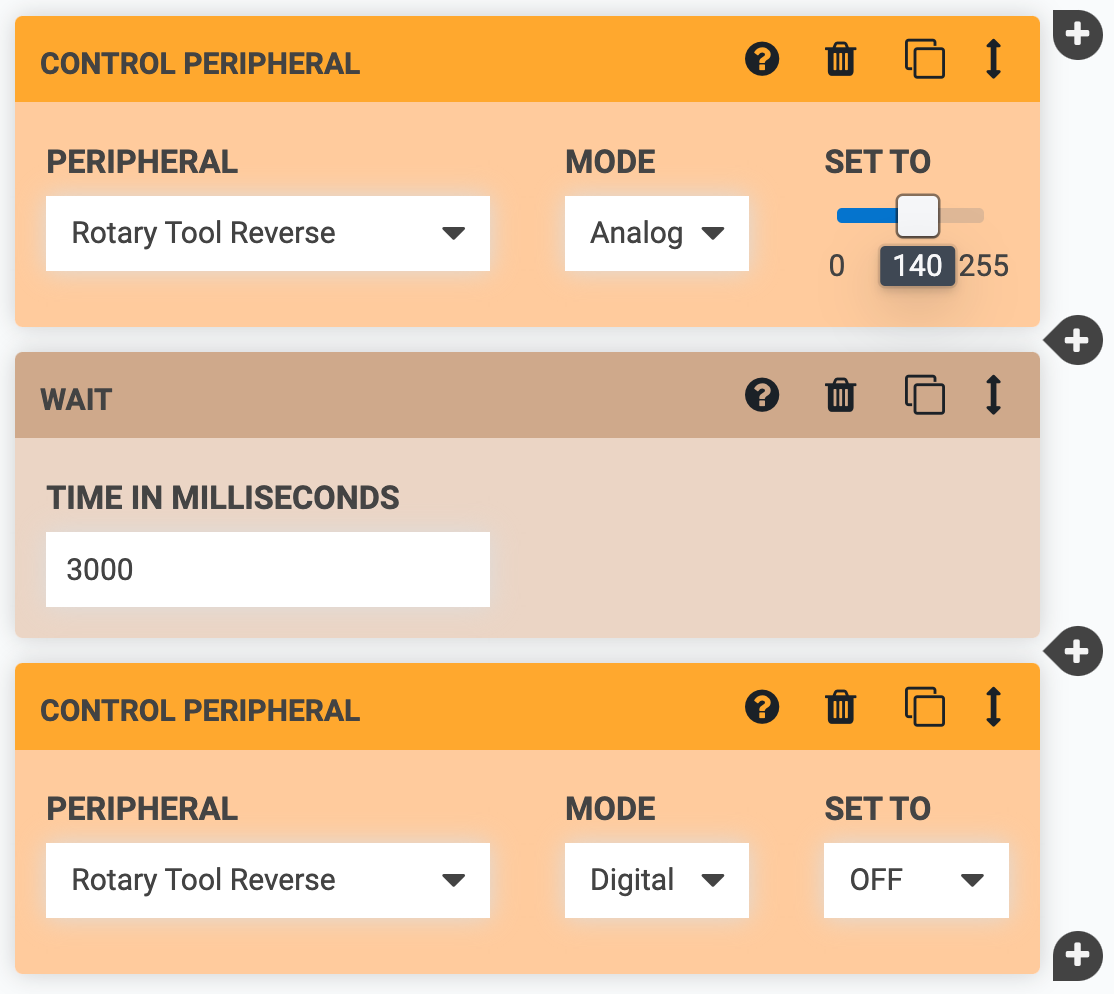
\includegraphics[width=0.6\linewidth]{Figures/ui_seq.png}
        \caption{Sequential Command}
        \label{fig:ui_seq}
    \end{figure}

    
    FarmBot Express's web application prioritizes user control over every aspect of their automated gardening experience. However, manual oversight of each individual action becomes impractical for large-scale or complex tasks. Sequences address this challenge by enabling users to combine fundamental FarmBot commands, such as movement and peripheral control, into structured, multi-step programs. These programs, exemplified by a sequence that retrieves a watering nozzle, hydrates a specific plant and then returns the nozzle to its storage position, automate intricate tasks and optimize user time management within their flourishing gardens.

    \textbf{Visualize farm data and sensor readings}
    
    \begin{figure}[H]
        \centering
        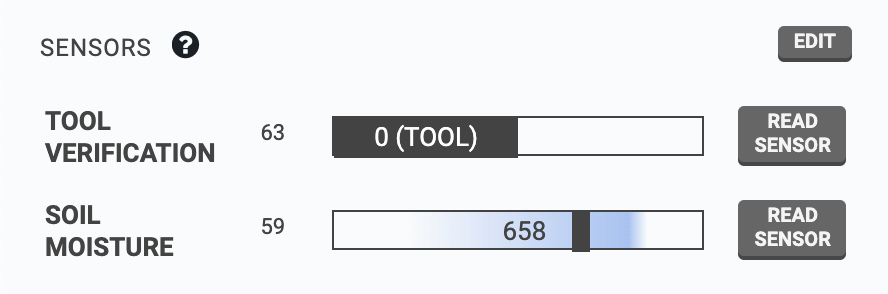
\includegraphics[width=0.6\linewidth]{Figures/ui_sensors.png}
        \caption{Sensor Configuration}
        \label{fig:ui_sensor}
    \end{figure}

    Users can easily access the sensor data using the web application of the FarmBot Express. This interface enables users to handle many harsh situations by providing user and cloud components with real-time data. 
    
\end{itemize}

\subsubsection{Hardware Interfaces}
Hardware interfaces define the physical connections between various hardware components within FarmBot Express. They specify the physical form (e.g., connectors, pins) and ensure proper electrical connections for data and power transfer. Examples include:

\begin{itemize}
    \item \textbf{Tool Head Interface:} This interface defines the physical connection between the robotic arm and the 3-in-1 tool head, allowing for easy attachment and detachment. This is a proprietary FarmBot design with a standard electrical connector.
    \item \textbf{Motor Control Interface:} This interface specifies the physical connection between the microcontroller and the FarmBot's motors. It ensures proper signal transmission for motor control.
\end{itemize}

\begin{figure}
    \centering
    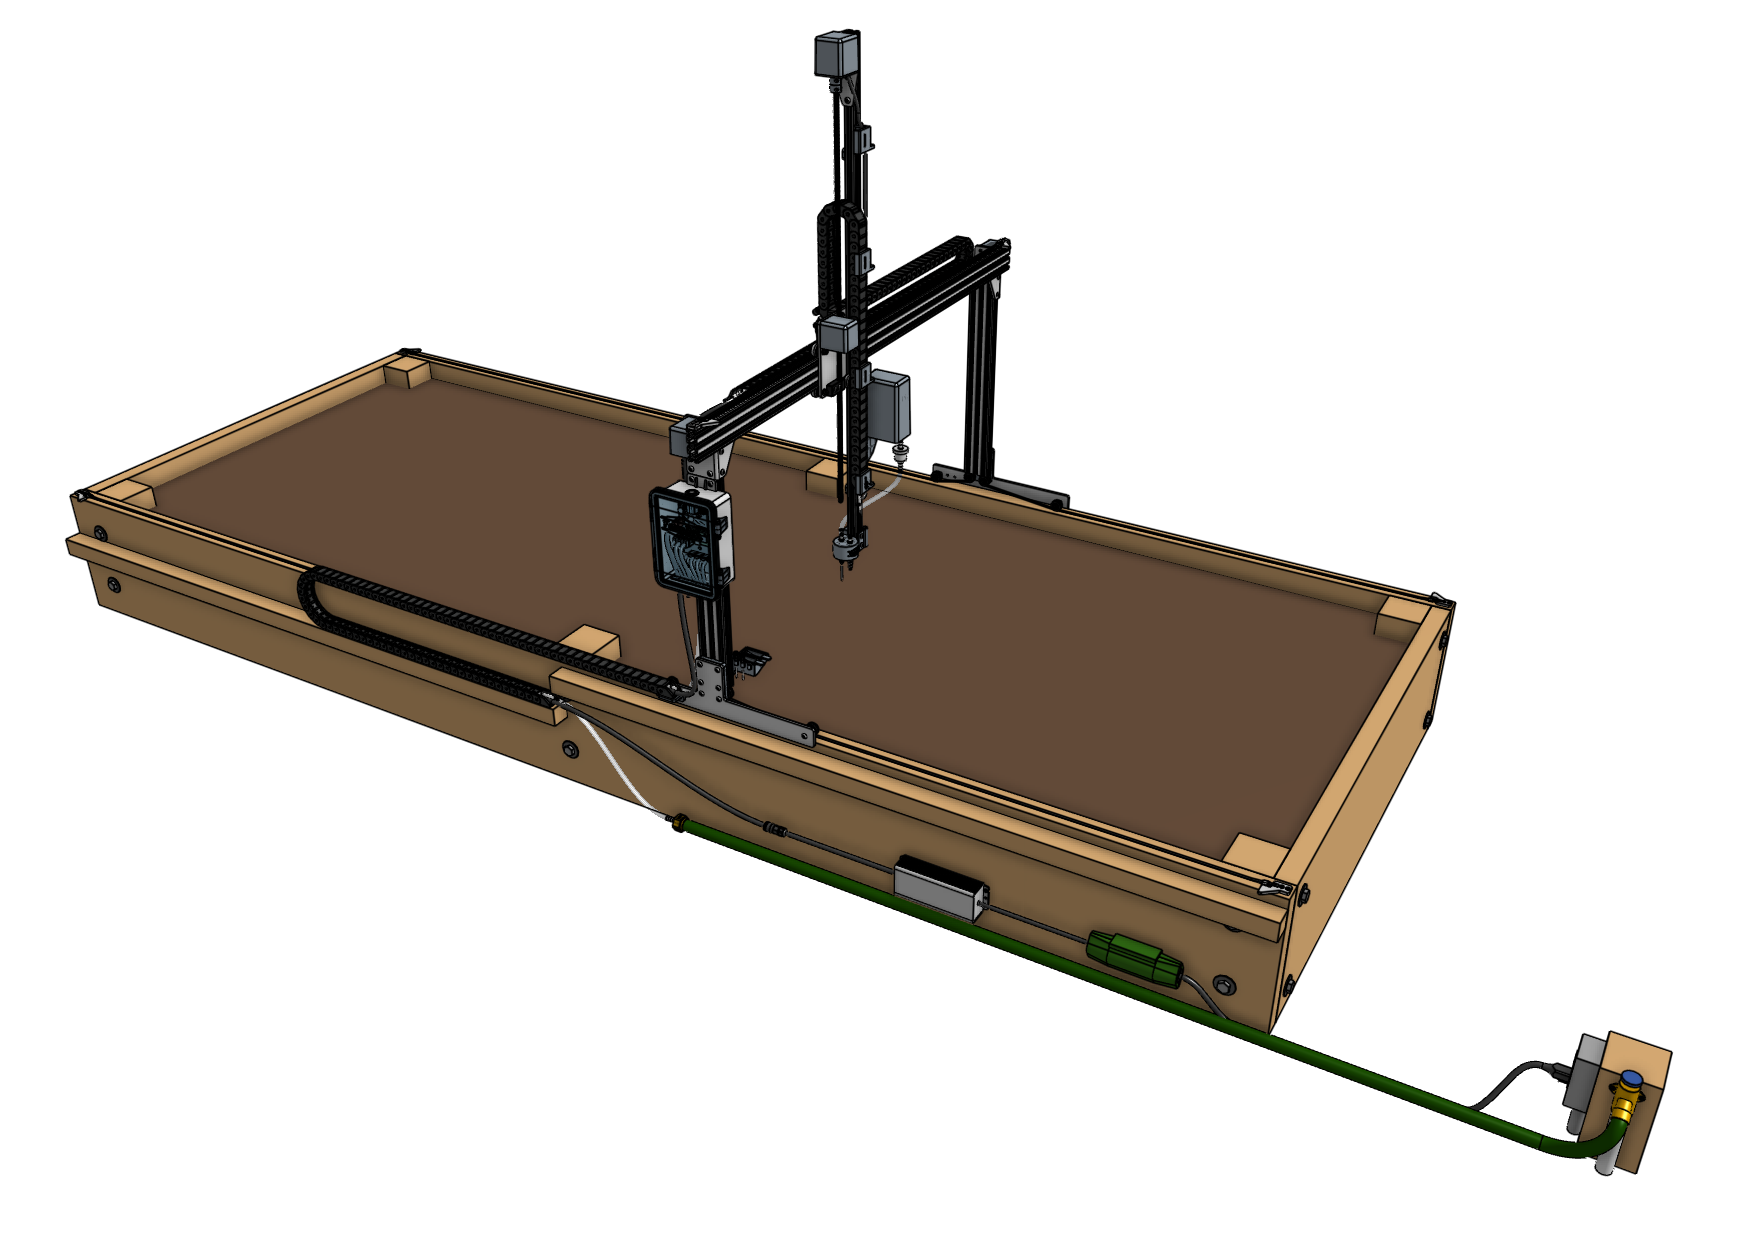
\includegraphics[scale=0.2]{Figures/farmbot_express_v1.1.png}
    \caption{FarmBot Express v1.1 Hardware}
    \label{fig:hardware}
\end{figure}

FarmBot combines user-friendly input with a mechanical design. While FarmBot utilizes a robotic arm and various tools to automate tasks, the user interacts with the system through a user-friendly interface, likely a web application or mobile app. This interface allows users to plan their garden layout, schedule planting and watering tasks, and monitor plant growth.  Essentially, the user interacts with FarmBot through a digital interface, while the physical actions in the garden are carried out by the mechanical components.

\subsubsection{Software Interfaces}
Software interfaces define the communication protocols and data formats used for software components to interact with each other. They specify the message structure, data types, and communication methods for seamless software interaction.
\begin{itemize}
    \item \textbf{Microcontroller Software Interface:}
    
    This software interface defines how the central computer (often a Raspberry Pi) communicates with the onboard microcontroller. It uses an operating system named FarmBot OS developed for FarmBot to translate digital instructions into motor control commands. The FarmBot's onboard microcontroller utilizes its own embedded operating system to interpret numerical code received from the backend software and transmit sensor data back online. This embedded system includes functionalities for code interpretation, sensor data acquisition (taking photos), and data communication (accepting real-time commands and uploading photos to a web application).
    \item \textbf{Sensor Data Interface and Arduino Firmware:}

    Sensor Data Interface: This software interface defines the data format and communication protocol sensors use to transmit data (e.g., soil moisture, and temperature) to the central computer. However, the crucial role of the Arduino firmware comes into play before this data reaches the central computer.\\
    \textbf{Arduino Firmware - The Bridge Between Sensors and FarmBot OS:}
    
    The firmware flashed onto the Arduino or Farmduino microcontroller acts as the bridge between the physical sensors and the FarmBot OS software running on the Raspberry Pi. Here's a breakdown of its functionalities:
    
    Sensor Data Acquisition: The Arduino firmware actively reads sensor data (soil moisture, temperature, etc.) through the physical pins connected to the sensors.
    Data Formatting and Communication: The firmware translates the raw sensor data into a specific format (potentially adhering to established protocols) suitable for transmission.
    Communication with FarmBot OS: The formatted sensor data, along with readings from rotary encoders and other pins, is then sent back to the Raspberry Pi running the FarmBot OS software. This communication likely occurs using G and F codes.

    \item \textbf{Backend Interface:}
    
    The Backend Interface serves as the backbone of FarmBot Express, facilitating seamless communication between the user-facing web interface and various internal software components. It acts as a central hub, managing essential data and functionalities:

    \textbf{User Management:}
    
    The interface handles user account creation, storage, and retrieval of user profile information. This ensures secure user authentication and facilitates personalized experiences within the FarmBot system. The more detailed version of user interaction and FarmBot's web application is argued in the User Interface part.
    
    \textbf{Farm Data Management:}
    
    This aspect of the interface focuses on all data associated with a user's farm. It allows creation, editing, and access to farm profiles, which encompass details like size, plant layouts, settings, scheduled operations, statistics, data maps, and farm history. Essentially, the backend interface serves as the repository for all farm-specific information.
    
    \textbf{Equipment Profiles:}
    
    The interface maintains information about the user's FarmBot hardware, including its current configuration and operational status. This ensures compatibility between uploaded control code and the actual capabilities of the equipment. Additionally, the interface facilitates updates to equipment profiles as configurations change due to upgrades, maintenance, or other reasons.
    
    \textbf{Decision Support System Interaction:}
    
    The backend interface bridges the gap between the user-facing elements and the decision support system, an algorithmic component responsible for optimizing farm operations. It enables data exchange between the decision support system and other backend components. This allows the system to access relevant farm data (plant information, sensor readings, etc.) to make informed decisions regarding planting, watering, and other farm management tasks.

    \begin{figure}[H]
        \centering
        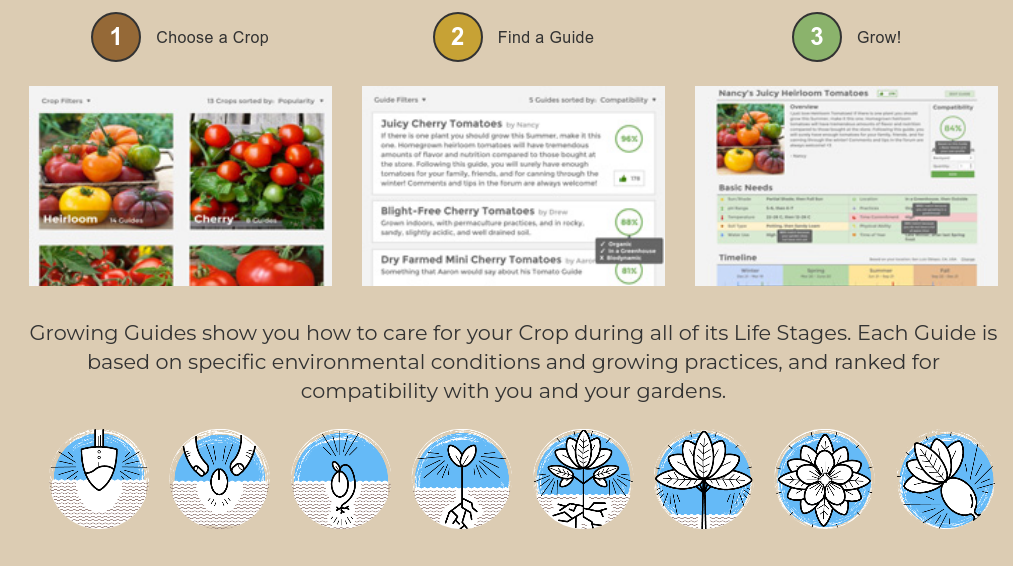
\includegraphics[width=0.85\linewidth]{Figures/openfarm_cc.png}
        \caption{OpenFarm.cc}
        \label{fig:openfarm}
    \end{figure}
    
    \textbf{Data Integration}
    
    While not explicitly mentioned as a core function of the Backend Interface, FarmBot Express might leverage cloud services to retrieve additional crop information from external databases like OpenFarm.cc. This integration enriches the decision support system by providing users access to a wider range of plant data for informed decision-making.
    
\end{itemize}


\subsubsection{Communication Interfaces}
Communication interfaces govern the exchange of data between FarmBot and external systems. They define the communication protocols and data formats used for internet connectivity, sensor data transmission, and potential future integrations. 
\begin{itemize}
    \item \textbf{Wi-Fi Interface:} This communication interface enables wireless communication between the central computer and the internet using the IEEE 802.11 standard (e.g., Wi-Fi b/g/n). This allows for remote user interaction and potential software updates.
\end{itemize}

\textbf{Communication Mechanisms:}

Communication between these interfaces occurs through the established protocols and data formats mentioned above. Here's a breakdown of some key communication mechanisms:
\begin{itemize}
    \item \textbf{Serial Communication:} This is a common method for communication between the central computer and the microcontroller. It involves sending data one bit at a time over a dedicated serial communication line. There exists a USB communication in between Farmduino to Raspberry Pi.
    \item \textbf{Network Communication:} The Wi-Fi interface utilizes network communication protocols defined by the IEEE 802.11 standard to connect FarmBot to the internet thanks to the operating system specially designed for the FarmBot Express Project, named FarmBot OS. This sophisticated mechanism provides the user many opportunities to interact with his farm. Furthermore, the Raspberry Pi has an integrated Wi-Fi radio antenna and an ethernet connector module. 
\end{itemize}

\textbf{Standardization and Benefits:}\\
By adhering to established communication protocols and utilizing standardized interfaces whenever possible (e.g., I2C, SPI, Wi-Fi), FarmBot ensures compatibility with readily available components. This facilitates future expansion with additional sensors or tools, allowing users to customize their FarmBot experience. Additionally, standardized communication protocols simplify troubleshooting and system maintenance.
\subsubsection{Memory Constraints}
\textbf{Technical Feasibility:} FarmBot Express leverages established technologies (Raspberry Pi, sensors, open-source software) and cloud integration, making it technically achievable for users with moderate technical knowledge. The cloud-based deployment of the decision support system significantly reduces memory constraints on the Raspberry Pi for FarmBot Express. The FarmBot software can focus on core functionalities with a moderate memory footprint, while the cloud handles intensive computations and data storage.

\textbf{Economic Feasibility:} While FarmBot Express offers automation and convenience, its cost-effectiveness depends on the user. It might be more suitable for hobbyists or small-scale gardeners who value these benefits.  Large-scale farms would need to assess cost savings (labor, yield) against traditional methods.

\textbf{Social Feasibility:}  FarmBot Express might require some technical knowledge for setup and operation, potentially limiting accessibility for non-tech-savvy users. However, it promotes water conservation and potentially reduces reliance on chemical pesticides through precise watering and weed management (with compatible attachments).

Overall, FarmBot Express is technically feasible, but economic and social factors require consideration. It caters well to home users and small-scale gardeners seeking automation, while larger operations need a cost-benefit analysis.


\subsubsection{Operations}

\begin{itemize}
    \item \textbf{System Operations:}
        \begin{itemize}
            \item Sow and water the seeds
            \item Monitoring the seeds
            \item Get crop data from database
            \item Guide for optimal design
            \item Scan garden and detect weeds
            \item Display logs
            \item Display external data
            \item Authentication
        \end{itemize}
    \item \textbf{User Operations:}
        \begin{itemize}
            \item Create custom farm design
            \item Create custom sequence models
            \item Log in to web application
            \item Save farm designs
            \item Customize external tools
        \end{itemize}
\end{itemize}

\subsection{System Functions}

Table 1.1 below, provides the system functions in tabulated manner. \\
\begin{longtblr}[
  label = none,
  entry = none,
]{
  width = \linewidth,
  colspec = {Q[363]Q[462]},
  hlines,
  vlines,
}
\textbf{Function} & Description \\
\textbf{Sow seeds, water and monitor} & The system sows seeds, waters them individually and monitors the garden. \\
\textbf{Customize farm design} & The system allows user to create custom farm designs through the web app via a simple drag-and-drop designer. \\
\textbf{Acquire crop data via external crop database} & The FarmBot Cloud Service communicates with the external crop database OpenFarm.cc, which provides crop information to the web app. \\
\textbf{Guide for optimal farm design} & The system guides the user for the most optimal farm design using the crop data available. \\
\textbf{Create custom sequences of farming actions} & The system allows the user to create custom sequences to run on the device, through the web app with a custom sequence editor. \\
\textbf{Scan garden and detect weeds} & The system scans the garden using cameras and computer vision algorithms, detecting weeds in a timely manner. \\
\textbf{Display system logs} & The system displays to the user, the logs of the device through the web app. \\
\textbf{Display sensor data} & The system displays to the user, the sensor data coming from the device through the web app. \\
\textbf{Display photos} & The system displays to the user, photos taken by the device's camera through the web app. \\
\textbf{Authenticate user} & The system authenticates the user by passing its web app credentials \\
\textbf{Save garden designs}  & The system saves designs created by the user for reusability. \\
\textbf{Customization of sensors, tooling} & The system firmware allows users to implement custom sensors and tooling on the device.
\end{longtblr}


\subsection{Stakeholder Characteristics}

The stakeholders of the system are range from students, researchers, robotic artwork creators, to home users, people with disabilities. Characteristics of the stakeholders are explained below:
\begin{itemize}
    \item \textbf{Students:} For students in any level of study from K12 (Kindergarten and grades 1-12) to university education, FarmBot provides a practical, fun and hands-on learning experience for STEM (Science, Technology, Engineering and Mathematics) learning objectives such as: \textbf{robotics}, \textbf{coding}, \textbf{soil science}, \textbf{biology}, and \textbf{much more}. They can be called novices in the domain of FarmBot. They do not have the necessary knowledge to fully comprehend the hardware-software interactions. They are naturally curious which encourages them to come up with new features, ways to use the device. They want to have the freedom to use their creativity. In addition to that, the students do not have a long attention span and it might be hard to keep them engaged.

    \item \textbf{Researchers:} For researchers, there are various ways to take advantage of the FarmBot. It offers repeatability, scale, speed, and low cost to researchers.
    \begin{itemize}
        \item \textbf{Repeatability}: The human error factor needs to be eliminated which leads to more accurate and repeatable results while experimenting. In addition, they want to schedule events (experiments) easily.
        \item \textbf{Scale}: Researchers want to easily test multiple groups of crops and run multiple experiments concurrently.
        \item \textbf{Speed}: Researchers want to create their own sequences and collect data automatically at any frequency, run experiments 24/7.
        \item \textbf{Cost}: Researchers want to avoid high labor costs
    \end{itemize}
    This class of stakeholders is highly educated therefore can capitalize on FarmBot being highly customizable, integratable. They would like to create custom tooling (eg. brush heads for coral farming), custom regimens (eg. for speeding up coral growth) for their experiments. Collecting accurate data in a timely fashion is of utmost importance to them. Precise and continous data flow from sensors, cameras free the researchers from labor intensive tasks and potential for error. This class uses FarmBot for \textbf{phenotyping research}, \textbf{photogrammetry}, \textbf{off-world farming research} and such.

    \item \textbf{Robotic Artwork Creators:} This class of stakeholders approach to using FarmBot is different from the others. Their perspective is more creative and artistic. They use the various sensors and cameras of the device, feed the data from them into different algorithms such as \textbf{stable diffusion} to create art pieces. For this class, ability to customize farm designs and sequence customizing are crucial features. They have, similar to the researchers class, the required knowledge of technology and they are generally well educated.  

    \item \textbf{Home User:} The home user class is usually driven to use FarmBot because of emerging problems in the world such as climate change, environmental pollution due to plastic packaging and excessive pesticide use. This class takes pride in being able to grow its food itself and being able to grow challenging plants. They are not experts on the technology, they have general knowledge. They usually use their backyards, small gardens for farming. They generally do not have a lot of spare time to tend to their garden each day.

    \item \textbf{People with disabilites:} These people suffer from various physical and mental limitations in their day-to-day lives. They are not able to farm on their own using conventional farming techniques (eg. can't clean the garden from weeds). Centres for disabled people can use FarmBot for horticultural therapy (the art or practice of garden cultivation and management) or vocational training. This would help them integrate with the society and give them a sense of autonomy. They do not have the technical expertise due to physical and mental handicaps. 

\end{itemize}

\subsection{Limitations}

\begin{itemize}
    \item \textbf{Regulatory Requirements:} {The FarmBot project is 100\% open-source. Hardware designs, software source code, and documentation are openly shared. However, technical support for DIY builds, customizations are not to be provided. In addition, FarmBot must comply with the local farming laws and regulations.}
    \item \textbf{Hardware Limitations:} {The custom electronics board needs a dedicated processor in order to monitor the rotary encoders at high speed and a Raspberry Pi 3 to be used as the brain communicating through the web. In addition, FarmBot has four stepper motors and needs to provide a tested rotary encoder for closed-loop feedback control. Lastly, FarmBot needs to be able to work with custom tooling.}
    \item \textbf{Interfaces to Other Applications:} {FarmBot must be able to communicate with external resources through its cloud services for crop information. Interacting with FarmBot from the web must be done using FarmBot.JS or FarmBot.Py and requests must be done according to the provided API.}
    \item \textbf{Parallel Operation:} {Parallel operation is crucial to FarmBot. It needs to be able to handle multiple crops of various types and sizes. Also, FarmBot needs to be able to handle data flow from sensors and cameras in parallel.}
    \item \textbf{Audit Functions:} {FarmBot web app handles user credentials and wifi credentials of the user. The way this data is stored and protected may require auditing from relevant organizations.}
    \item \textbf{Control Functions:} {Since FarmBot is an open-source project, the control function does not exist. In contrast to being central, it is distributed to the community.}
    \item \textbf{Higher-order Language Requirements:} {The frontend for the web application is developed using TypeScript and ReactJS UI library. The backend is developed using Ruby on Rails, and PostgreSQL. Google Cloud is used for file storage. The message broker sub-component is built as a custom RabbitMQ instance. CeleryScript is used for handling data exchange between systems in an asynchronous and predictable way. Elixir is used to develop FarmBot OS to handle low level details. Lastly, the firmware for Arduino is written in C++ to communicate effectively with the hardware.}
    \item \textbf{Signal Handshake Protocols:} {HTTPS is used for communication between client and server, therefore SSL Handshake Protocol is used.}
    \item \textbf{Quality Requirements:} {Precision, scalability, automation, space efficiency, continuous land use, ease of customization are important quality requirements of FarmBot.}
    \item \textbf{Criticality of the application:} {The FarmBot system is not critical. The effects of system failure would not be drastic.}
    \item \textbf{Safety and Security Considerations:} {The user and wifi credentials must be stored safely. Also, the device shall not harm the user while executing actions.}
    \item \textbf{Physical/Mental Considerations:} {The user must be able to at least interact with the drag-and-drop no-code programming environment and must have the basic physical and mental capability to set up the device.}
    \item \textbf{Limitations that are sourced from other systems, including real-time requirements
from the controlled system through interfaces:} {The FarmBot system communicates with the crop database OpenFarm as an external resource. This information shall be updated regularly. In addition, the system shall also communicate with user devices such as laptops, mobile phones and data flow must be real-time. For example, taking pictures from the camera or sensor data logs.}
\end{itemize}

\section{Definitions}
\begin{itemize}
    \item HTTPS: Hypertext Transfer Protocol Secure (HTTPS) is an extension of the Hypertext Transfer Protocol (HTTP). It uses encryption for secure communication over a computer network, and is widely used on the Internet.
    \item SSL: SSL, or Secure Sockets Layer, is an encryption-based Internet security protocol.
    \item API: A set of functions and procedures allowing the creation of applications that access the features or data of an operating system, application, or other service.
    \item I2C: Inter-Integrated-circuit (I2C) is a simple, bidirectional two-wire synchronous serial bus that requires only two wires to transmit information between devices connected to the bus. 
    \item SPI: Serial Peripheral Interface (SPI) is a de facto standard (with many variants) for synchronous serial communication, used primarily in embedded systems for short-distance wired communication between integrated circuits.
\end{itemize}
